%&pdflatex
\chapter{Results}

\section{Data Acquisition \& Preprocessing}
[Describe data preprocessing and its results]

[Yes this needs to be larger, no I do not yet know how.]
Prior to the join operation, the mixing matrix consisted of 10817 samples and after 8862 were left. [numbers are results]

\section{Validation \& Performance}
[Describe how you ensured the validity of the outcomes of your own methodologies and code.]
[Uuuhm, partially maybe software tests? Apart from that, trusting the implementations made by people way smarter than me?]

\section{Research results}
The actual results

\subsection{Generalised Linear Models using Elastic Net Regularisation} \label{sec:results:glmnet}
[Was first in methods. Rewrite to be more appropriate for results]
A model with the settings in \fref{tab:glmnet_conv_reg} did not converge. Increasing the maximum number of iterations, \verb|maxit|, up to hundredfold and the convergence threshold, \verb|thresh|, up to thousandfold did not help.
When the elastic net mixing parameter \verb|alpha| was set to anything but one (representing lasso regularisation) the model did converge, but performance was dismal.
The predicted probabilities contained NaN values, which shouldn't ever happen.

However, when the elastic net mixing parameter \verb|alpha| was set to anything but one (lasso regularisation) the model did converge.
Unfortunately, performance of this model was dismal, and the predicted probabilities contained \verb|NaN| values.

In an attempt to circumvent this issue, cancer types with fewer than one hundred samples were removed from the dataset before the split into training, testing, and validation data.
This reduced the total number of cancer types from 28 to 22 cancer types.
This relatively simple change stopped the model from converging at all, no matter the regularisation method.

In order to simplify the problem a subset with 250 randomly chosen samples from two randomly chosen cancer types was made.
Of this subset 70\% of samples, or 175 samples, were put in the training set.
If the model converged, a cancer types would be added to the subset, of which 250 samples would be randomly chosen again, resulting in \fref{fig:glmnet_conv_reg}
%&pdflatex
\begin{figure}[htp]
    \centering
    \textbf{This is a beautiful figure title}\par\medskip
    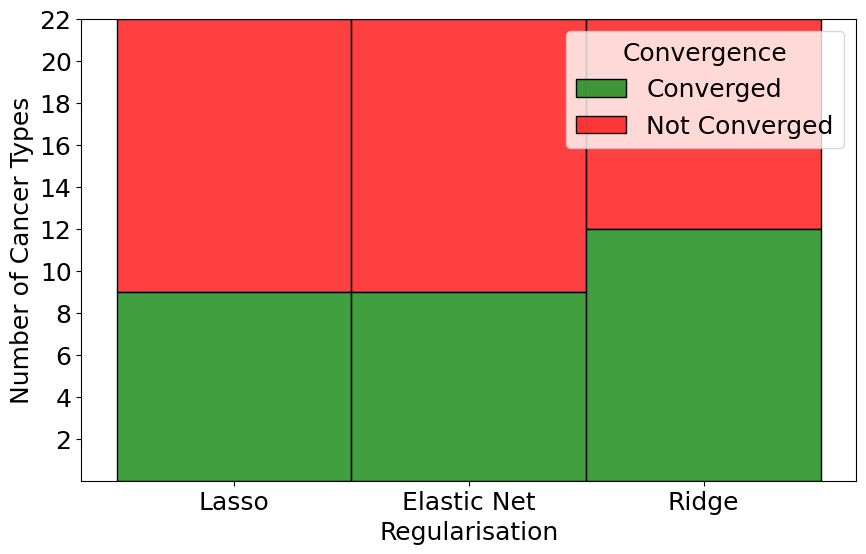
\includegraphics[scale=0.45]{glmnet_conv_reg_18pt}
\caption{blablabla}
\label{fig:glmnet_conv_reg}
\end{figure}

[note that captions should explain everything about a figure]


While convergence was achieved, this implementation worked with just over half the cancer types in the dataset.
To achieve convergence with more cancer types the issue of class imbalance was addressed.
A subset where every cancer type has exactly 100 randomly chosen samples in the training set was created.
All remaining samples were put into a testing subset.

As before, convergence was checked with two randomly chosen cancer types and, if the model converged, another cancer type would be added to the subsets.
However, this resulted in the same outcome as \fref{fig:glmnet_conv_reg}.

[Not sure where to put this or if to include this:]
Given that the model stops converging when the number of cancer types is greater than twelve, the twelfth through twenty-second cancer types were aggregated into a single "other" label.
This model did not converge.

Since the model did converge when the training set contained 100 samples for each of twelve cancer types ...

Thus far the number of cancer types has been the subject of change, while the number of samples per cancer type may be adjusted as well.
Continuing from the best working configuration where each of twelve cancer types had 100 samples in the training set, the latter value was adjusted downward.
This resulted in the following:
%&pdflatex
\begin{figure}[htp]
    \centering
    \textbf{This is a beautiful figure title}\par\medskip
    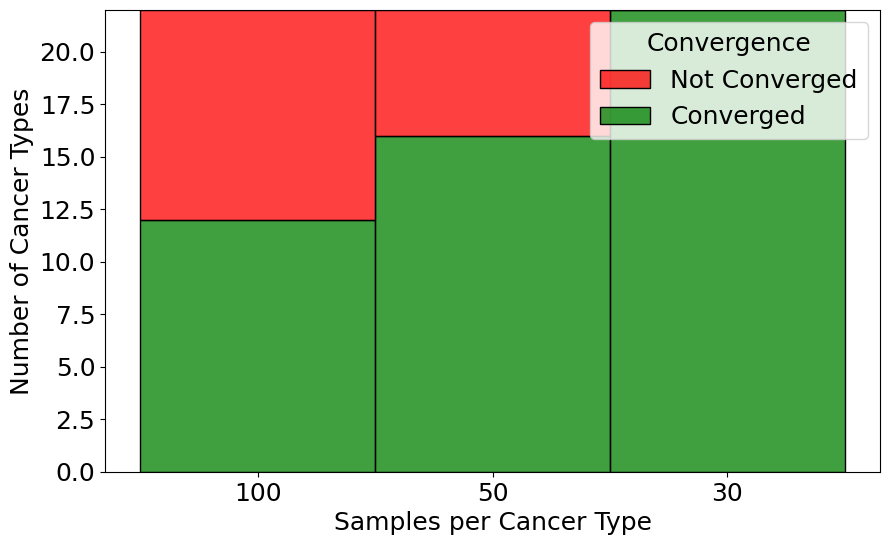
\includegraphics[scale=0.45]{glmnet_conv_18pt}
\caption{Explain everything about the figure here. What colour is what? What do the names in the legend mean? One should understand the entire figure by just reading the caption, without needing to read the rest of the text.}
\label{fig:glmnet_conv}
\end{figure}


In order the optimise performance and utility, the training set should contain the maximum number of samples per cancer type while also using as many cancer types as possible.
As can be seen in \fref{fig:glmnet_conv}, there is an optimal number between thirty and fifty samples per cancer type when using all twenty-two cancer types.
An optimum of 32 samples per cancer types was found by increasing the number of samples per cancer type by one at a time while checking if the model would still converge.

To summarise the following method was used:
\begin{itemize}
    \item Remove cancer types with fewer than 100 samples from the dataset.
    \item Create a training set where each cancer type has 32 samples. Place the remaining samples in the testing set.
    \item Run \verb|cv.glmnet| with parameters found in \fref[plain]{tab:glmnet_conv_reg}.
    \item Run \verb|glmnet| with parameters found in \fref[plain]{tab:glmnet_conv_reg}.
\end{itemize}

Although this method works, it leaves the majority of the dataset unused for the model's training process.
Therefore, another more versatile type of model was needed.

\subsection{Conditional Inference Trees}
%&pdflatex
\begin{table}[htp]
    \centering
    \begin{tabular}{|p{2cm}|p{2cm}||p{1cm}|p{1cm}|p{1cm}|p{1.2cm}||p{1cm}|p{1cm}|p{1cm}|p{1.2cm}|}
        \hline
        \multicolumn{2}{|c||}{\textbf{Settings}} & \multicolumn{8}{|c|}{\textbf{Performance Metrics}}  \\
        \hline
        \multicolumn{2}{|c||}{} & \multicolumn{4}{|c||}{\textbf{Train}} & \multicolumn{4}{|c|}{\textbf{Test}} \\
        \hline
        \hline
        \textbf{minsplit} & \textbf{minbucket} & \textbf{AUC} & \textbf{MCC} & \textbf{ARI} & \textbf{Top-3} & \textbf{AUC} & \textbf{MCC} & \textbf{ARI} & \textbf{Top-3} \\
        \hline
        10 & 7 & 0.9991 & 0.9301 & 0.8817 & 0.9911 & 0.9566 & 0.8734 & 0.8045 & 0.9367 \\
        \hline
        20 & 7 & 0.9989 & 0.9234 & 0.8704 & 0.9909 & 0.9593 & 0.8703 & 0.7977 & 0.9420 \\
        \hline
        30 & 7 & 0.9986 & 0.9141 & 0.8541 & 0.9895 & 0.9627 & 0.8687 & 0.7931 & 0.9465 \\
        \hline
        20 & 3 & 0.9995 & 0.9504 & 0.9135 & 0.9958 & 0.9406 & 0.8798 & 0.8076 & 0.9240 \\
        \hline
        20 & 14 & 0.9978 & 0.8952 & 0.8245 & 0.9854 & 0.9541 & 0.8664 & 0.7854 & 0.9443 \\
        \hline
    \end{tabular}
    \caption{Ctree gridsearch small. Maybe convert to plots?}
    \label{tab:ctree_gs}
\end{table}


%&pdflatex
\begin{figure}[htp]
    \centering
    \textbf{This is a beautiful figure title}\par\medskip
    \begin{subfigure}[b]{.3\textwidth}
        \centering
        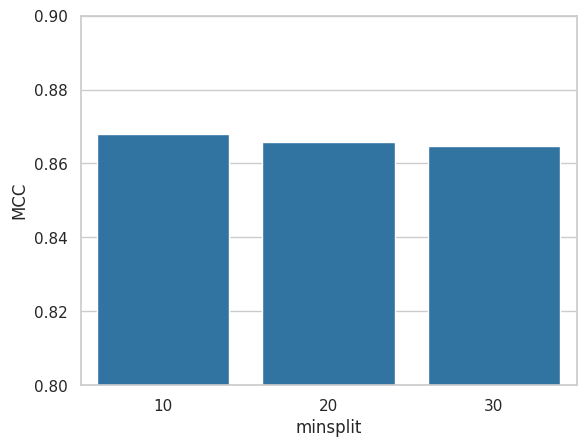
\includegraphics[scale=0.6]{ctgss_mcc_minsplit}
        \cprotect\caption{MCC versus \verb|minsplit|}
        \label{fig:ctgss_mcc_minsplit}
    \end{subfigure}
    \hfill
    \begin{subfigure}[b]{.3\textwidth}
        \centering
        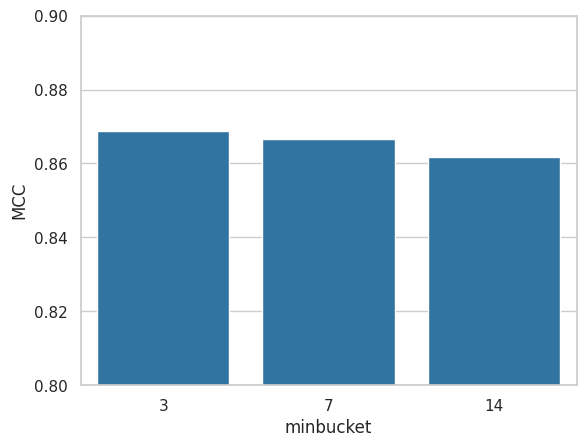
\includegraphics[scale=0.6]{ctgss_mcc_minbucket}
        \cprotect\caption{MCC versus \verb|minbucket|}
        \label{fig:ctgss_mcc_minbucket}
    \end{subfigure}
    \hspace*{\fill}

    \caption{Results of gridsearch for ctree.}
\end{figure}


A low value for minbucket and around the middle value for minsplit seem pretty good.

\subsection{Conditional Inference Forests}
%&pdflatex
\begin{table}[htp]
    \centering
    \begin{tabular}{|p{1.5cm}|p{2cm}|p{2cm}||p{1cm}|p{1cm}|p{1cm}|p{1.2cm}||p{1cm}|p{1cm}|p{1cm}|p{1.2cm}|}
        \hline
        \multicolumn{3}{|c||}{\textbf{Settings}} & \multicolumn{8}{|c|}{\textbf{Performance Metrics}}  \\
        \hline
        \multicolumn{3}{|c||}{} & \multicolumn{4}{|c||}{\textbf{Train}} & \multicolumn{4}{|c|}{\textbf{Test}} \\
        \hline
        \hline
        \textbf{ntrees} & \textbf{minsplit} & \textbf{minbucket} & \textbf{AUC} & \textbf{MCC} & \textbf{ARI} & \textbf{Top-3} & \textbf{AUC} & \textbf{MCC} & \textbf{ARI} & \textbf{Top-3} \\
        \hline
        10 & 10 & 7 & 0.9995 & 0.9614 & 0.9384 & 0.9980 & 0.9948 & 0.9123 & 0.8610 & 0.9811 \\
        \hline
        10 & 20 & 7 & 0.9994 & 0.9554 & 0.9306 & 0.9970 & 0.9962 & 0.9210 & 0.8819 & 0.9811 \\
        \hline
        10 & 30 & 7 & 0.9992 & 0.9435 & 0.9117 & 0.9956 & 0.9957 & 0.9163 & 0.8751 & 0.9849 \\
        \hline
        10 & 20 & 3 & 0.9997 & 0.9723 & 0.9547 & 0.9991 & 0.9919 & 0.9130 & 0.8720 & 0.9811 \\
        \hline
        10 & 20 & 14 & 0.9987 & 0.9339 & 0.8948 & 0.9927 & 0.9937 & 0.9070 & 0.8451 & 0.9819 \\
        \hline
        50 & 20 & 7 & 0.9997 & 0.9643 & 0.9441 & 0.9998 & 0.9975 & 0.9306 & 0.8957 & 0.9909 \\
        \hline
    \end{tabular}
    \caption{Cforest gridsearch small. Maybe convert to plots?}
    \label{tab:cforest_gs}
\end{table}


%&pdflatex
\begin{figure}[htp]
    \centering
    \textbf{This is a beautiful figure title}\par\medskip
    \begin{subfigure}[b]{.3\textwidth}
        \centering
        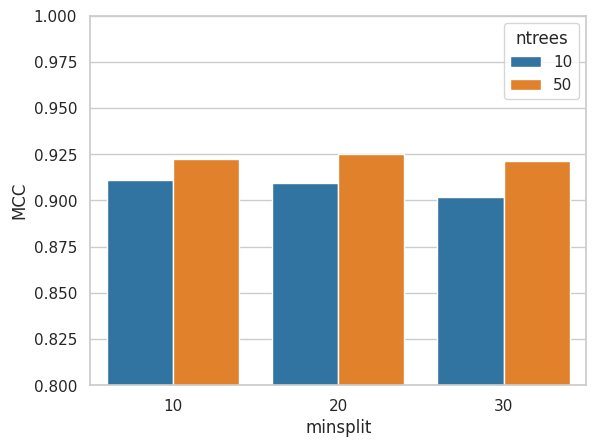
\includegraphics[scale=0.6]{cfgss_mcc_minsplit}
        \cprotect\caption{MCC versus \verb|minsplit|}
        \label{fig:cfgss_mcc_minsplit}
    \end{subfigure}
    \hfill
    \begin{subfigure}[b]{.3\textwidth}
        \centering
        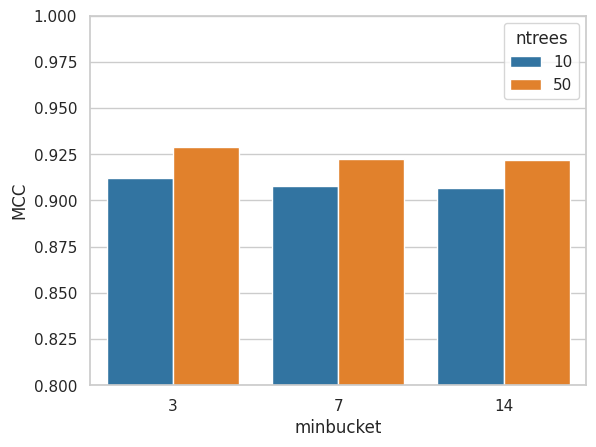
\includegraphics[scale=0.6]{cfgss_mcc_minbucket}
        \cprotect\caption{MCC versus \verb|minbucket|}
        \label{fig:cfgss_mcc_minbucket}
    \end{subfigure}
    \hspace*{\fill}

    \caption{Results of gridsearch for cforest.}
\end{figure}


Still need to rerun the one that didn't work.
More trees produce the best results.
Apart from that results seem fairly consisten with ctree.

%&pdflatex
\begin{figure}[htp]
    \centering
    \textbf{This is a beautiful figure title}\par\medskip
    % \hspace*{\fill}
    \begin{subfigure}[b]{.3\textwidth}
        \centering
        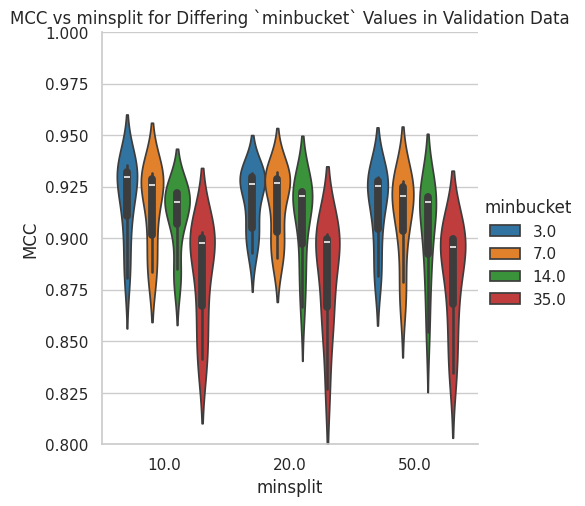
\includegraphics[scale=0.45]{cfgsl_mcc_minsplit_violin}
        \cprotect\caption{MCC versus \verb|minsplit| for varying values for \verb|minbucket|}
        \label{fig:cfgsl_mcc_minsplit_violin}
    \end{subfigure}
    \hfill
    \begin{subfigure}[b]{.3\textwidth}
        \centering
        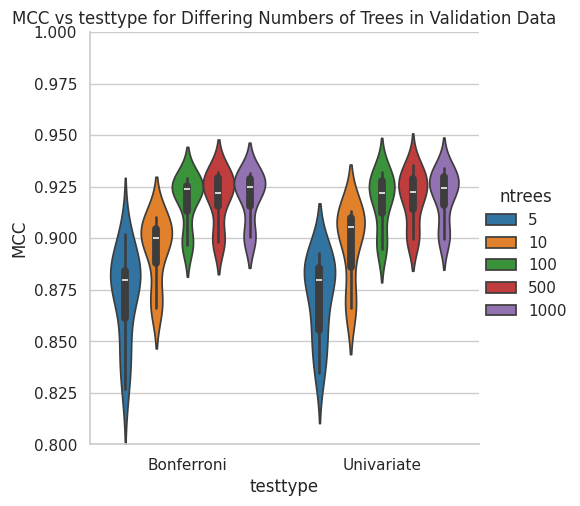
\includegraphics[scale=0.45]{cfgsl_mcc_testtype_violin}
        \cprotect\caption{MCC versus \verb|testtype| for varying numbers of trees.}
        \label{fig:cfgsl_mcc_testtype_violin}
    \end{subfigure}
    \hspace*{\fill}

    \begin{subfigure}[b]{.3\textwidth}
        \centering
        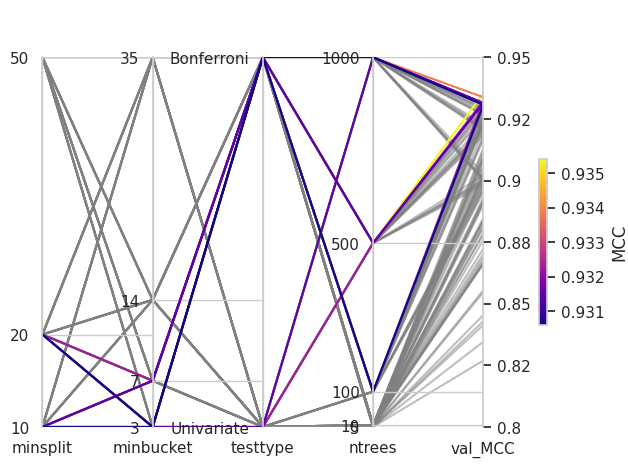
\includegraphics[scale=0.45]{cfgsl_pc}
        \caption{Top 10 forests by MCC}
        \label{fig:cfgsl_pc}
    \end{subfigure}
\caption{Results of gridsearch for the best hyperparameters for cforest.}
\end{figure}

Observing \ref{fig:cfgsl_mcc_minsplit_violin} shows a lower minbucket value tends to result in a higher MCC.
The same figure also shows that MCC scores stay fairly stable across different minsplit values.
[Can I say these things without having a statistical test backing up whether they are actually different or the same?]


Figure \ref{fig:cfgsl_mcc_testtype_violin} shows a clear pattern of higher numbers of trees resulting in higher MCC scores with the increase flattening after 100 trees.

Might not include \ref{fig:cfgsl_pc} because it looks confusing, and I'm not sure what to say about it.

\subsection{Model Selection}
Picked the model with the highest MCC at [x]. This model was trained with the following parameters.

%&pdflatex
\begin{table}[H]
    \centering
    \begin{tabular}{|p{3cm}|p{3cm}|}
        \hline
        \textbf{Metric} & \textbf{Value} \\
        \hline
        \hline
        \texttt{testtype} & Univariate \\
        \hline
        \texttt{ntrees} & 1000 \\
        \hline
        \texttt{minsplit} & 10 \\
        \hline
        \texttt{minbucket} & 3 \\
        \hline
    \end{tabular}
    \caption{this is a caption}
    \label{tab:cforest_best_metrics}
\end{table}


\subsection{Validation on Microarray Data}
Using the best conditional inference forest thus far to predict cancer types of samples from the GPL570 dataset resulted in the performance metrics found in [...].

More like a decrease in performance metrics across the board as compared to performance on the mRNA expression profiles.

[insert performance metrics]
[insert heatmap]
[insert sad face]
[insert dist of top 3 probabilities]
[insert plot of difference between best and second-best probability]
Looks like the model is having difficulty distinguishing between the two labels with the highest probability.

\subsection{Variable Importance}
[Something like "the top x most important TCs account for x\% of the mean decrease in accuracy."]
